\section{Resultados e Discussões}

\subsection*{Parte 1}

Os dados obtidos estão mostrados na tabela \ref{tab: exp1}. 
O valor médio encontrado para $\lambda$ foi $\langle \lambda \rangle = 633 \pm 26  \text{ nm} $, o que equivale a um desvio de 0,03$\%$ do valor informado pelo fabricante de 632,8 nm. Esse valor foi utilizado para os cálculo

\begin{table}[h]
\centering
\caption{Medidas do primeiro experimento.}
\begin{tabular}{c|c|c|c}
\toprule\midrule
$x_0$ (mm)& $x_1$ (mm) & $\Lambda$ ($\mu$m) & $\lambda$ (nm) \\
\midrule
0,45 & 0,62 & 34 & 567 \\
2,41 & 2,61 & 40 & 667 \\
7,13 & 7,32 & 38 & 633 \\
7,65 & 7,85 & 40 & 667 \\
9,21 & 9,40 & 38 & 633 \\
\midrule\bottomrule
\end{tabular}
\label{tab: exp1}
\end{table}

\subsection*{Parte 2}

Os dados obtidos estão mostrados na tabela \ref{tab: exp2}. Utilizando o software Grace para fazer uma regressão linear, mostrada na Fig. \ref{fig: regression}, foi encontrado o coeficiente linear $0,035479$ mbar$^{-1}$. Utilizando esse resultado na eq. \eqref{eq: kappa}, obtemos

\begin{equation*}
\begin{aligned}
\kappa &= \frac{(633 \times 10^{-9} \text{ m})}{2(4,1 \times 10^{-2} \text{ m})} (0,035470 \times 10^{3} \text{ mbar}^{-1}) \\ 
&= 2,74 \times 10^{-4} \text{ bar}^{-1}\;.
\end{aligned}
\end{equation*}

\begin{table}[b]
\centering
\caption{Dados do segundo experimento. Os valores da primeira coluna são adimensionais, os outros estão em mbar.}
\begin{tabular}{ccccccccccccc}
\toprule\midrule
$m$ & $P_{1}$ & $P_{2}$ & $P_{3}$ & $P_{4}$ & $P_{5}$ & $P_{6}$ & $P_{7}$ & $P_{8}$ & $P_{9}$ & $P_{10}$ & $\langle P \rangle$ & $\Delta P$\\
\midrule
5 & 220 & 220 & 200 & 220 & 210 & 220 & 200 & 220 & 220 & 220 & 215 & 7 \\
10 & 380 & 380 & 360 & 370 & 380 & 380 & 360 & 380 & 380 & 380 & 375 & 7 \\
15 & 540 & 540 & 520 & 520 & 520 & 520 & 500 & 530 & 540 & 530 & 526 & 10 \\
20 & 680 & 680 & 650 & 660 & 660 & 660 & 640 & 670 & 680 & 680 & 666 & 12 \\
25 & 780 & 770 & 780 & 780 & 760 & 760 & 740 & 780 & 780 & 770 & 770 & 10 \\
\midrule\bottomrule
\end{tabular}
\label{tab: exp2}
\end{table}

\noindent Tendo obtido $\kappa$, basta fazer $p = 1 \text{ bar}$ na eq. \eqref{eq: n(p)} para obter o valor de $n_{ar}$ à pressão atmosférica:

\begin{equation*}
\begin{aligned}
n_{ar} &= 1 + (2,74 \times 10^{-4} \text{ bar}^{-1})(1 \text{ bar}) \\
&= 1,000274 \;,
\end{aligned}
\end{equation*}

\noindent o que está de acordo com o valor informado pela literatura, de 1,000273 \ccite{wiki}, com um desvio percentual $<0,0001 \%$.

\begin{figure}[t]
\centering
\caption{Regressão linear dos dados do experimento 2. }
\includegraphics[width=0.8\columnwidth]{imagens/regression.eps}
\small{\\Fonte: Autor, 2026.}
\label{fig: regression}
\end{figure}


\begin{table}[h]
\centering
\caption{Medidas do terceiro experimento.}
\begin{tabular}{c|c|c}
\toprule\midrule
$m$ & $\theta$ ($^\circ$) & $n$ \\
\midrule   
40 & 6.7 & 1.8592 \\ 
40 & 6.8 & 1.8135 \\ 
60 & 8.8 & 1.6695 \\ 
60 & 8.6 & 1.7243 \\ 
60 & 8.4 & 1.7872 \\ 
60 & 8.6 & 1.7243 \\    
\midrule\bottomrule
\end{tabular}
\label{tab: exp3}
\end{table}

\subsection*{Parte 3}

Os dados obtidos estão mostrados na tabela \ref{tab: exp3}. O valor médio encontrado para $n$ foi $\langle n \rangle = 1,76 \pm 0,06$, que está no limite da faixa de valores dada pela literatura (entre 1,4 e 1,8).




